\begin{figure}[!htp]
    \centering
    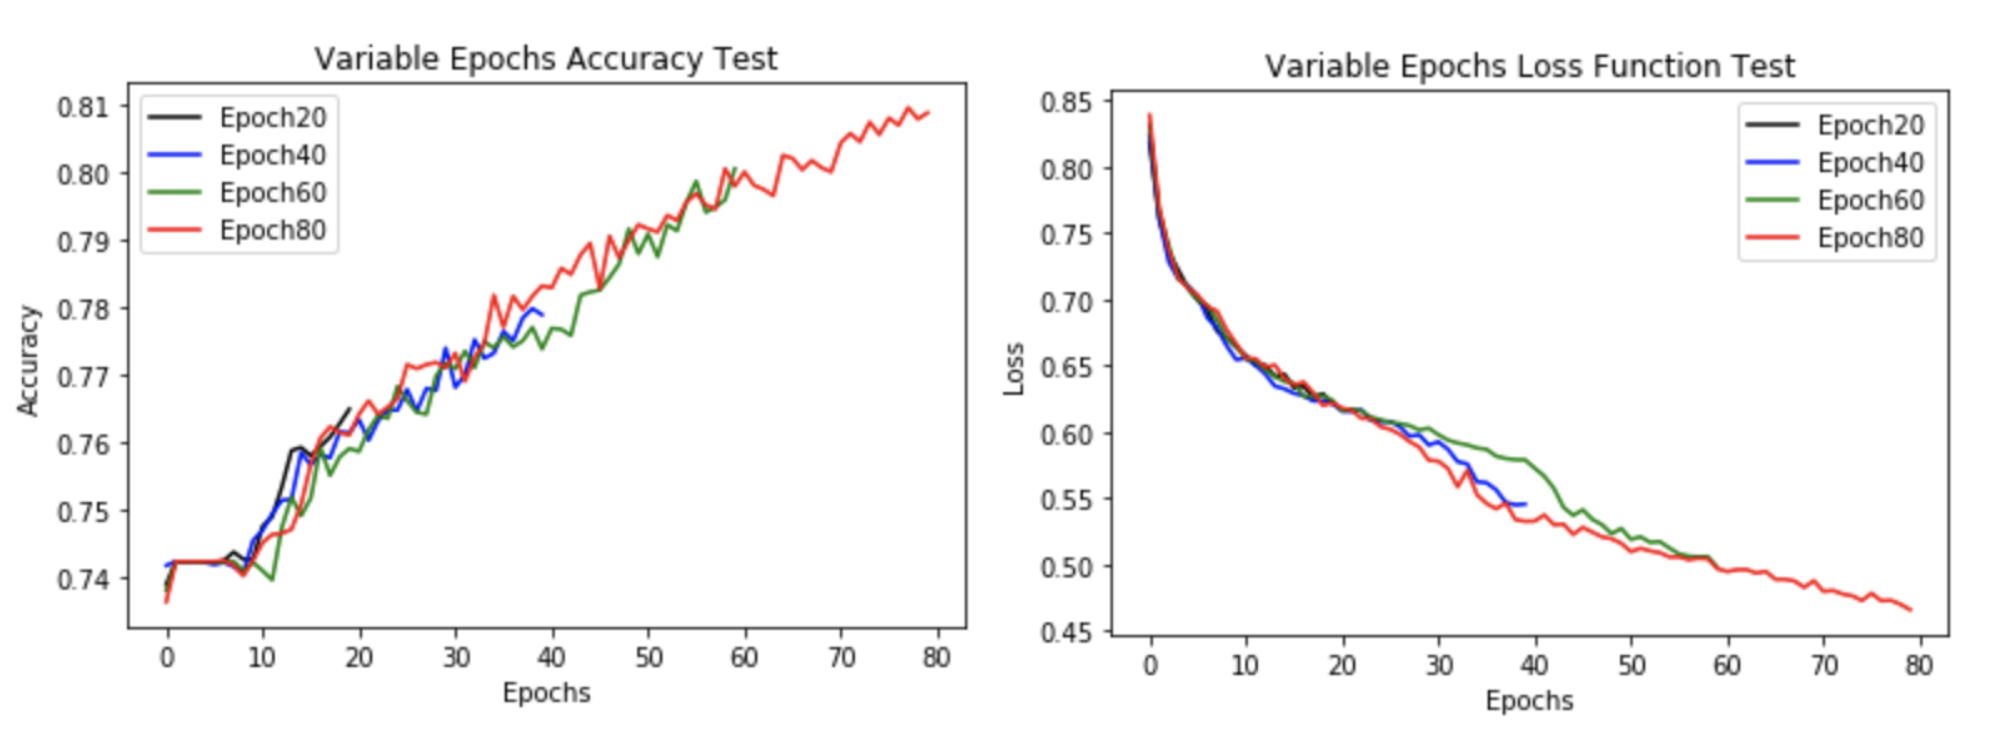
\includegraphics[width=15cm]{Images/epochs.png}
    \caption{Variable Epochs}
    \label{fig:epochs}
\end{figure}

The figure \ref{fig:lrates} above shows that the model was trained for different learning rates as shown
in the legend of the figure \ref{fig:lrates} for thirty epochs or iterations. The outcome of the above test 
was that the model model accuracy of the model were increasing with decrease in the learning rates. Thus, it 
can be concluded that the model accuracy was  inversely proportional to the learning rate. The figure \ref{fig:lrates} also shows the 
decline in the loss function where learning rate was found directly proportional to loss function of the 
convolutional model. Therefore, the most optimal learning rate to train the convolutional network 
neural network was 0.0001. However, the model with the lower the learning rate consumes more time in the 
process of training. Further model training experiments are peformed on 
learning rate of 0.001 to achieve the accuracy and realtive speed to train the model.
\pagebreak

\begin{center}
    \begin{tabular} {| c | c | c |}
        \hline
        Learning Rate & Test Accuracy & Epochs \\ 
        \hline
        0.1 & 74.5\% & 30 \\ 
        \hline 
        0.01 & 77.6\% & 30  \\
        \hline 
        0.001 & 74.2 & 30  \\
        \hline
        0.0001 & 75.2 & 30  \\
        \hline
    \end{tabular}
\end{center}

